\chapter{Imágenes BIAS y DARK}
\setcounter{ipythcntr}{0}

El primer tipo de imágenes con las que trabajaremos son las imágenes de bias y las de corriente oscura. En este documento se presenta un resumen de ambos casos, para más detalles dirígete a los Notebooks \norbash{Example-1-BIAS.ipynb} y \norbash{Example-1-DARK.ipynb}. Los datos que usaremos se encuentran en la siguiente enlace: \url{https://zenodo.org/records/3254683}. Debes descargar el archivo y descomprimirlo en tu misma carpeta de trabajo para que las rutas mostradas en los Notebooks funcionen. 

\section{El módulo ccdproc}
Como se mencionó anteriormente, el módulo que se utiliza en Python para la reducción de datos astronómicos es \pynorm{ccdproc}. Para instalarlo, simplemente escribe \bashbold{pip install ccdproc} en la terminal cuando tu entorno de Python esté activado.

El módulo \pynorm{ccdproc} permite combinar archivos de bias, dark current y flat fields, además de corregir las imágenes de objetos por cada una de estas fuentes de ruido. Las imágenes combinadas de cada tipo suelen denominarse "master" (master bias, master dark, master flat). En esta clase aprenderemos a crear este tipo de archivos.

Es importante tener en cuenta que cada análisis de datos CCD es único. Los pasos que revisaremos para este conjunto de datos son apropiados para el instrumento específico, pero podrían no ser aplicables a otros telescopios o instrumentos. Para determinar los pasos adecuados en cada caso, es fundamental conocer la naturaleza de los datos y su organización. En realidad, el aprendizaje de la reducción de datos es una cuestión de práctica y experiencia. Por ello, cuando utilicemos IRAF, trabajaremos con datos de otro instrumento, de modo que puedas ver que, aunque los principios básicos son los mismos, cada procedimiento varía según el instrumento y las características de los datos.

\subsection{Creando un archivo master bias}
Este ejemplo está basado en la guía <<\href{}{CCD Data reduction guide}>> de Python. Los datos corresponden al instrumento <<Large Field Camera>> (LFC) del Observatorio de Palomar. Los datos se encuentran dentro de la carpeta llamada \pynorm{'example-cryo-LFC'} y dentro de ella existen imágenes de bias, dark y flat. Comencemos leyendo un archivo de cada tipo:

\begin{pyin}
from ccdproc import CCDData, ImageFileCollection
from pathlib import Path
import numpy as np
from astropy.stats import mad_std
\end{pyin}

\begin{pyin}[]
#- Definiendo la ruta a los datos
cryo_path = Path('example-cryo-LFC')

#- Leyendo unas cuantas imágenes
bias_lfc   = CCDData.read(cryo_path / 'ccd.001.0.fits', unit='count')
object_lfc = CCDData.read(cryo_path / 'ccd.037.0.fits' , unit='count')
flat_lfc   = CCDData.read(cryo_path / 'ccd.014.0.fits', unit='count') 
\end{pyin}

El CCD de este instrumento cuenta con una sección llamada <<\emph{overscan}>>, que consiste de una parte cubierta del CCD. Se trata de una región adicional que no corresponde a ninguna parte de la imagen física, sino a píxeles ficticios que se utilizan para medir y corregir el nivel de bias. Los detalles técnicos del LFC pueden encontrarse en su \href{https://sites.astro.caltech.edu/palomar/observer/200inchResources/lfcspecs.html}{página oficial}, donde se muestra que sus imágenes cuentan con $ 2048 \times 4096 $ pixeles. Sin embargo, cuando leemos los datos nos damos cuenta que existen pixeles extra, los cuales conforman el overscan:

\begin{pyin}[]
#- Obteniendo la cantidad de pixeles
bias_lfc.shape
\end{pyin}
\begin{pyout}
(4128, 2080)
\end{pyout}

\begin{figure}[htb]
  \centering
				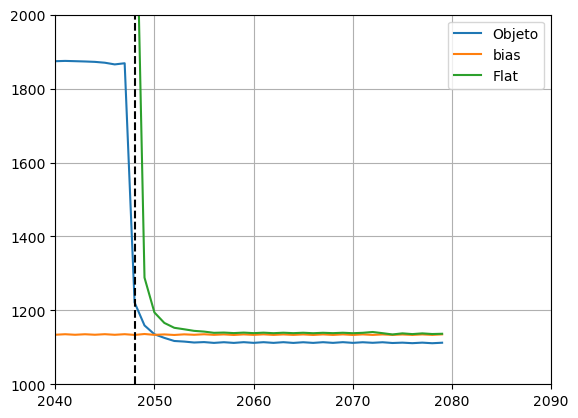
\includegraphics[width=0.7\textwidth]{figures/overscan.png}
				\caption{Intensidad con respecto a los pixeles}
				\label{fig:overscan} 
\end{figure}

Al hacer un gráfico de la intensidad de la señal con respecto a cada pixel obtenemos lo mostrado en la Figura \ref{fig:overscan}. Lo que observamos es que a partir del pixel 2048, la señal detectada para el objeto y para las imágenes flat comienzan a disminuir y eventualmente alcanzan la misma intensidad que las imágenes de bias. El hecho de que se observe esta caída y que además se mantiene constante nos indica que sí podemos utilizar la información que nos brinda el overscan. Lo que debemos hacer es restar el valor constante que se alcanza luego del pixel $ \gtrsim 2048 $ a todas nuestras imágenes, con eso estaríamos al mismo tiempo corrigiendo por bias. 

Primero debemos crear una carpeta donde colocaremos las imágenes a las que aplicaremos esta corrección. Preferiblmente deberá estar ubicada en tu mismo directorio de trabajo. Puedes por ejemplo llamar a esta carpeta \pynorm{'example-reduced'} y crearla de la siguiente manera:

\begin{pyin}[]
#- Crea una nueva carpeta
calibrated_data = Path('.', 'example-reduced')
calibrated_data.mkdir(exist_ok=True)
\end{pyin}

Ahora creamos una colección de archivos con todas las imágenes dentro de la carpeta \pynorm{'example-cryo-lfc}. Esta colección tendrá las imágenes bias, flat y las de objeto.
\begin{pyin}
files = ImageFileCollection(cryo_path)
\end{pyin}

Para quedarnos únicamente con las de bias, que son las que nos interesan por el momento, debemos filtrarlas con una de las funciones dentro del módulo \pynorm{ImageFileCollection}. Dicha función se llama \pynorm{files_filtered()} y podemos usarla de la siguiente manera:

\begin{pyin}[]
#- Seleccionando solo imágenes tipo bias
biases = files.files_filtered(include_path=True, imagetyp='BIAS')
\end{pyin}

Para entender qué es lo que haremos con todas estas imágenes, primero aplicaremos el procedimiento a una sola imagen y veremos el resultado. Comencemos seleccionando la primera imagen de nuestra lista:

\begin{pyin}[]
#- Seleccionando una sola imagen
first_bias = CCDData.read(biases[0], unit='adu')
\end{pyin}

Como vemos en la Figura \ref{fig:overscan}, a pesar que el overscan de este instrumento inicia a partir del píxel 2048, la intensidad se mantiene constante para los tres tipos de imágenes a partir del píxel 2055 aproximadamente. Por lo tanto, debemos sustraer ese valor de intensidad a nuestra imagen. Primero importamos la función que nos permite realizar esa tarea:

\begin{pyin}
from ccdproc import subtract_overscan
\end{pyin}

Para estos datos específicos, la usamos de la siguiente manera:

\begin{pyin}
bias_overscan_substracted = subtract_overscan(first_bias, 
                                       overscan=first_bias[:, 2055: ],
                                       median=True)
\end{pyin}

Ahora debemos recortar la imagen para no utilizar los píxeles extra y quedarnos solo con los píxeles físicos. Primero importamos la función que utilizaremos:

\begin{pyin}
from ccdproc import trim_image
\end{pyin}

Y la utilizamos: 

\begin{pyin}
trimmed_bias = trim_image(bias_overscan_substracted[ :, :2048])
\end{pyin}

En la Figura \ref{fig:bias_compared} se compara la imagen inicial, llamada \pynorm{first_bias} y la imagen final, llamada \pynorm{trimmed_bias}. Como puedes notar, se redujo la intensidad de la imagen además que en el eje horizontal ahora hay menos píxeles. 

\begin{figure}[htb]
  \centering
	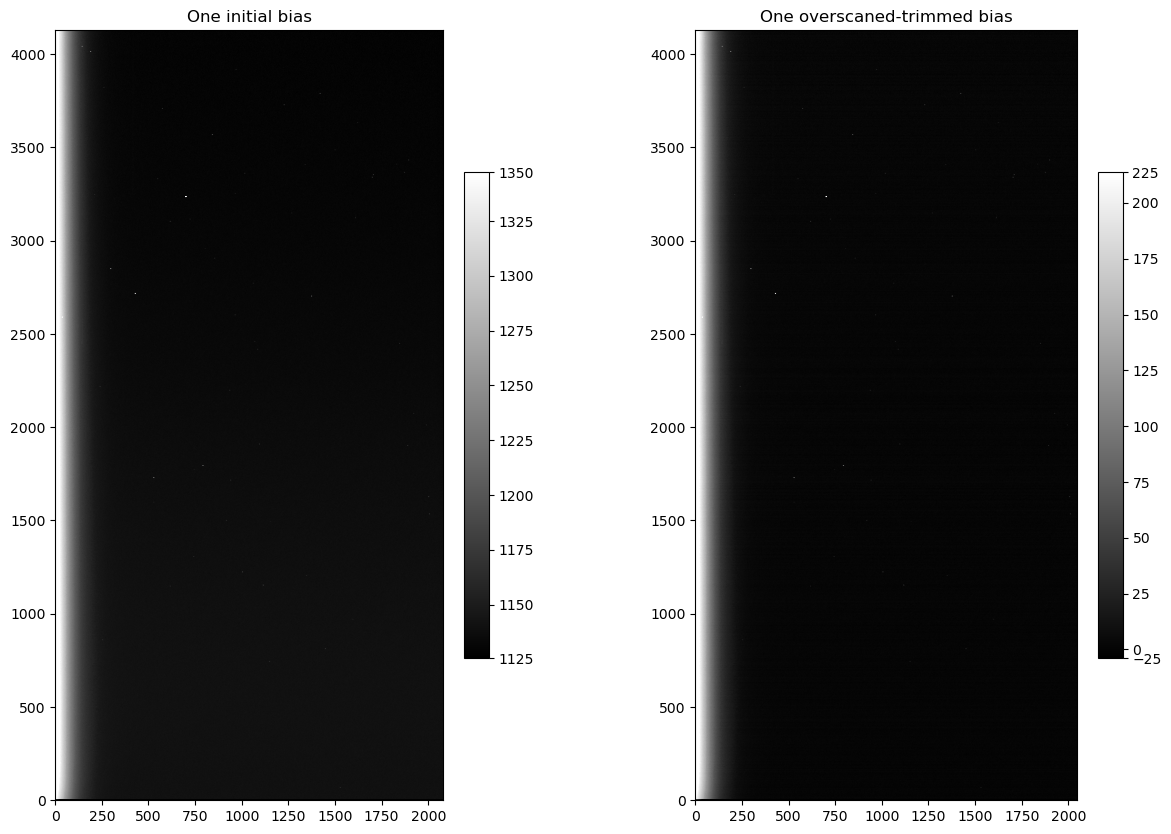
\includegraphics[width=0.45\textwidth]{figures/first_bias.png}
	\caption{Comparación de una imagen de bias antes y después de sustraer el overscan.}
	\label{fig:bias_compared} 
\end{figure}

Ahora que hemos comprendido el resultado de este procedimiento, podemos aplicarlo a todas las imágenes de bias usando un ciclo \pynorm{for}:

\begin{pyin}
for ccd_file, file_name in files.ccds(imagetyp='BIAS', 
                                      ccd_kwargs={'unit': 'adu'}, 
                                      return_fname=True):

    #- Restar el oberscan
    ccd_file = subtract_overscan(ccd_file, 
                                 overscan=ccd_file[: , 2055:], 
                                 median = True)

    #- Recortar los archivos
    ccd_file = trim_image(ccd_file[:, :2048])

    #- Guardar el resultado
    ccd_file.write(calibrated_data / file_name )
\end{pyin}

Con los datos corregidos, vamos a crear un archivo master bias, que es simplemente un promedio de todas las imágenes de bias. Primero seleccionamos las imágenes que acabamos de corregir:

\begin{pyin}[]
#- Creando una colección de imágenes
reduced_images = ImageFileCollection(calibrated_data)

calibrated_biases = reduced_images.files_filtered(imagetyp='bias', 
                                                  include_path=True)
\end{pyin}

Para crear el master bias, debemos usar la función \pynorm{combine()} del módulo \pynorm{ccdproc}. Primero la importamos:

\begin{pyin}
from ccdproc import combine
\end{pyin}

La utilizamos de la siguiente manera:

\begin{pyin}[]
#- Creando un master bias
combined_bias = combine(calibrated_biases,
                        method='average',
                        sigma_clip=True, sigma_clip_low_thresh=5,
                        sigma_clip_high_thresh=5,
                        sigma_clip_func=np.ma.median, 
                        sigma_clip_dev_func=mad_std,
                        mem_limit=350e6
                        )
\end{pyin}

Actualizamos la información del archivo y además lo guardamos:
\begin{pyin}[]
#- Actualizando la meta data
combined_bias.meta['combined'] = True

#- Guardando el archivo
combined_bias.write(calibrated_data / 'master_bias.fits')
\end{pyin}

\subsection{Creando un archivo master dark}
Para crear el archivo master dar, primero debemos sustraer el overscan y recortar las imágenes de dark current. Ya hemos definido la variable \pynorm{cryo_path} como la ubicación de nuestros archivos. Dentro de esa ubicación se encuentra el directorio llamado \pynorm{darks}. Para acceder a esos archivos, por lo tanto, debemos definir esa ruta:

\begin{pyin}[]
#- Ruta a las imágenes dark
lfc_darks_raw = ImageFileCollection(cryo_path / 'darks')
\end{pyin}

Aplicamos el mismo ciclo \pynorm{for} a todas las imágenes dark para restarles el overscan y recortarlas:

\begin{pyin}
for ccd, file_name in lfc_darks_raw.ccds(imagetyp='DARK',            
                                         ccd_kwargs={'unit': 'adu'},
                                         return_fname=True           
                                        ):    
    # Subtract the overscan
    ccd = subtract_overscan(ccd, overscan=ccd[:, 2055:], 
                            median=True)
    
    # Trim the overscan
    ccd = trim_image(ccd[:, :2048])
    
    # Save the result
    ccd.write(calibrated_data / file_name, overwrite=True)
\end{pyin}

Ahora debemos actualizar nuestra colección de imágenes reducidas:

\begin{pyin}
reduced_images.refresh()
\end{pyin}

Las imágenes dark tienen diferentes tiempos de exposición, por lo que debemos crear un archivo master dark para cada uno de ellos. Primero creamos un set con dichos tiempos:

\begin{pyin}
darks = reduced_images.summary['imagetyp'] == 'DARK'
dark_times = set(reduced_images.summary['exptime'][darks])
print(dark_times)
\end{pyin}
\begin{pyprint}
{300.0, 70.0, 7.0}
\end{pyprint}

Ahora usamos un ciclo for que itera sobre cada tiempo de exposición y luego:
\begin{itemize}
  \item Selecciona todas las imágenes dark para el tiempo de exposición dado
  \item Combina esas imágenes dark
  \item Actualiza su información
  \item Guarda los archivos combinados
\end{itemize}

\begin{pyin}
for exp_time in sorted(dark_times):

    #- Selecciona las imágenes dark dentro de la carpeta
    calibrated_darks = reduced_images.files_filtered(imagetyp='dark',
                                                     exptime=exp_time,
                                                     include_path=True)

    #- Combina las imágenes
    combined_dark = combine(calibrated_darks,
                            method='average',
                            sigma_clip=True, sigma_clip_low_thresh=5,
                            sigma_clip_high_thresh=5,
                            sigma_clip_func=np.ma.median, 
                            sigma_clip_dev_func=mad_std,
                            mem_limit=350e6
                            )

    #- Actualiza la información
    combined_dark.meta['combined'] = True

    #- Guarda los archivos
    dark_file_name = 'combined_dark_{:6.3f}.fits'.format(exp_time)
    combined_dark.write(calibrated_data / dark_file_name)
\end{pyin}

Con esto hemos creado los tres archivos master dark, uno para cada tiempo de exposición. 
